
\chapter{Generalization Error and Model Selection }\label{cha:modelSelection}

%\section{ Model Selection}\label{section-modelSelection}


\section{Prediction and Generalization Error}\label{subsection-generalizationError}

Given that in supervised learning settings, the goal is to build a learner with low predictive error, the algorithm's generalization power will then lie on its ability to correctly label new samples which wasn't used in the training phase. Measuring and comparing this ability among models is needed to select the best supervised estimator.
% of independent test data from $\mathrm{T_s}$

For now, let us assume that $f: X \rightarrow Y$ is a function which interacts the true existent relationship in the data: $Y = f(X) + \epsilon$. In this mapping from feature to target space we also assume $\epsilon$ to be the noise, with $0$ mean and fixed $\sigma^2$ variance i.e.\ $\epsilon \sim \calN(0,1) $. Then the equation in \cref{eq:rss} can be read as an approximation of the expected prediction error given the training set $\mathcal{T}$.


\begin{definition}{Prediction Error:}
	Given a loss function $L(\cdot,\cdot)$ and a function $f$, we say that the \textbf{prediction error} for the resulting classifier $f$ is
	\[
	PE(f_\theta)= \left[ L(\textbf{Y},f(\textbf{X}))\right]
	\]
\end{definition}

This is the error between our model transformation and the target labels, as quantified by the loss function.  In our specific example, with the parameters $\theta$ encoding the structure of $f$ as $f_\theta(x) = h(x \cdot \theta)$ we would that that:

\begin{definition}{Squared Loss Prediction Error:}
	Given a choice of parameter $\theta$ and the \textit{squared error loss}, we say that the \textbf{prediction error} for the resulting classifier $f_\theta$ is

	\begin{equation}
	PE_{true}(\theta) =L(\textbf{y} - h(\textbf{x} \cdot \theta) )  \\
	=  {(\textbf{y} - h(\textbf{x} \cdot \theta) )}^2
	\end{equation}

\end{definition}

Our interest is now in minimizing this error for all possible values. We would like to quantify the expected error over all random occurrences of $\textbf{X}$ and $\textbf{Y}$. This is known as the generalization error and is very related to the prediction error as it is its expectation.

\begin{definition}{Generalization Error:}
\begin{equation}
Err = \Expect_{ \textbf{X}, \textbf{Y} } \left[ L(Y,f(X)) \right]
\end{equation}
\end{definition}

Given that any model is always built on a dataset, we are required to estimate the generalization error using only the model's error over the data.
% $\mathcal{T_s}$:


\begin{equation}
	Err_{\mathcal{T}} = \Expect_{\textbf{X},\textbf{Y}} \left[ L(Y,\hat{f}(X)) | \mathcal{T}\right] \\
	= \int_{\mathcal{T}} {(y - h(x \cdot \theta) )}^2 P(x,y)dxdy
\end{equation}

	%\begin{equation}
	%  Err_{true}(\theta) = \Expect[(\textbf{y} - h(\textbf{x} \cdot \theta) )^2] \\
	%  = \int (y - h(x \cdot \theta) )^2 P(x,y)dxdy
	%\end{equation}

Note that in this definition the expectation is taken conditional on the training set and also from which the model is built.

%\begin{equation}
% PE = \Expect_{X,Y} \left[ L(Y,\hat{f}(X))\right] = \Expect \left[ Err_{\mathcal{T}} \right]
% \end{equation}.

In practice we have finite access to samples, so we have to estimate the generalization error. As such, we will have data to build or \textit{train} our model. From this reduced sample we will extract a training error to determine how well the model is performing. This will be our approximated prediction error through the
\begin{definition}{Training Error:}
	is the average loss over the sample prediction errors:
	$$ \overline{err}_{\mathcal{T}} = \frac{1}{N} \sum_{i=1}^N L(y_i, \hat{f}(x_i) )$$
\end{definition}\label{def:trainingError}

Let \textbf{x} $\in \mathbb{R}^{p}$ denote a random input variable and \textbf{y} $\in \mathbb{R}$ denote a random output variable with joint distribution $P\left(\textbf{x},\textbf{y}\right)$.

We will then turn to evaluate models according to their performance errors on $\mathcal{T}$ and $\mathcal{T_s}$ Combinations of high or low values for these, across training and test data, are used as model evaluation and highlight aspects to be improved.

\section{Bias, Variance and Systematic Values}\label{subsection-biasVariance}	If we look closer at the generalization error in our specific case of the squared loss function with

\begin{equation}\label{squaredPE}
EPE = \Expect_X \Expect_{Y|X} \left[ \left\Vert Y - \hat{f}(X) \right\Vert_2^2 \right]
\end{equation}

It is not difficult to see that the model that minimizes this error is $\hat{f}(x) = \Expect \left[ Y | X=x \right] $. Take Our model $\hat{f}$ to be an estimate of the true relation in the data, constructed from the data.

With the squared loss, the prediction error $\Expect \left[ \left\Vert Y - \hat{f}(X) \right\Vert_2^2 \right]$ of this model can be decomposed in the following way:

\begin{equation}\label{squaredBiasDecomposition}
\begin{split}
PE( \hat{f} ) = & {\Expect_X \left[  f(X) - \hat{f}(X) \right]}^2 + \Expect_X \left[ {\hat{f}(X)}^2 \right] \\
& - {\Expect_X \left[ \hat{f}(X) \right] }^2 + \sigma^2 \\
= & {Bias(\hat{f})}^2 + Var(\hat{f}) + \sigma^2
\end{split}
%= Bias(\hat{f})^2 + Var(\hat{f}) + \sigma^2
\end{equation}


Equation \cref{squaredBiasDecomposition} is hereby designated as the \textit{bias-variance decomposition for the squared loss}. The first term is called the square of the bias of the estimator. It measures how well off are our estimator's predictions compared to the true relational function. On the other hand, the second and third terms are the variance of the estimator. This will measure how this random variable varies along its most expected non-random value. The noise's variance term is that part of the prediction error which is irreducible. Note that we have already taken the expectation over the target and that is why we are left with the target's noise. This part of the error we cannot minimize or control with our learner. It is due to the random nature of the problem.

Note that integration here is done over the joint distribution of inputs and outputs. As we've mentioned before, we have incomplete information on $P(x,y)$ given the finite data $ \mathcal{T}$.
We must assume then that calculating this integral is not possible for any $\theta$ and must rely on estimation procedures.

For example, we could try and sample $M$ i.i.d.\ points from $P(x,y)$ to approximate the integral by a Monte Carlo scheme such as

\begin{equation}\label{eq:mcarlo-approx}
Err_{true}(\theta) \approx \frac{1}{M} \sum_i^M {( y - h(x \cdot \theta) )}^2
\end{equation}

Yet this would be unfeasible as well. Since the sampling process should be done for each specific $\theta$. Notice however the close resemblance of this equation \cref{eq:mcarlo-approx} to the form in \cref{eq:rss}.

Historically the errors due to bias and variance where associated directly with the squared loss function.  Yet in classification problems, the residual sum of squares is not the loss function used to estimate the model\'s parameters. Instead, they rely on other \textit{loss} functions that we will introduce later.

For this, we use a simple series approximation

\begin{equation}
Err_{train}(\theta) \approx  \Expect_{ \mathcal{T}}[{(y - h(x \cdot \theta) )}^2]
\end{equation}

%, and can be decomposed into two types of errors



In the literature such as \textcite{james-biasVarianceGeneral}, authors point to two sources responsible for this error, namely the bias and the variance of the learner. And the improvement of one generally leads to a hinder on the other. These errors are key elements in the prediction error because they point to different weak points in the algorithms. This in turn leads to different ways of tackling each error. To better improve the performance of an algorithm, controlling both is a key issue.

Conceptually the bias error represents the model's accuracy in labeling predictions correctly. It is the model's best attempt to capture the functional relationship among the feature and target variables. This could either mean it is correctly assigning the sample to its correct class in classification settings, or by predicting correctly the sample's target value in a regression setting.

The bias is lower when models correctly learn the underlying structures of the data. However, as bias decreases, the model complexity increases and more data is needed to train it correctly because the model becomes very fit to the training set i.e.\ it loses the ability to extend this predictive accuracy to new samples because they it learns too much from the available samples only. In this situation, we have another type of error which is known as an increase in variance.

In the generalization error, the loss function determines how \textit{good} the model's prediction are by quantifying these errors. Given a training set $\mathcal{T} = (X,Y)$, let $\hat{f}(X)$ be the model's predictive function for the features and denote $L( Y,\hat{f(X)} )$ the loss function acting on this data.

By comparing for each sample the target predictions versus their actual values, loss functions give a measure of how strong classifiers are with respect to their predictions. These can be described as semi metrics on the target space i.e.\ functions that are symmetric, non-negative and equal to zero only if both arguments are equal.

%{\huge \textbf{UNCOMMENT PROOFS, DEFINITIONS AND THEOREMS}}

We can extend the notion of bias and variance to loss functions more general than the squared loss error. This is explained in \textcite{james-biasVarianceGeneral}. The author defines what properties should be displayed by the bias and variance of an estimator. And for this we need to define the systematic value of a random variable with respect to a loss function.


\begin{definition}{Systematic Value:}
Given a training set $\mathcal{T}$, a loss function $L(\cdot)$ and a random variable $Z$, the systematic value or systematic component of this variable is
$$ SZ =  \argmin_u \Expect_{Z} \left[ L(u,Z) \right]$$
\end{definition}

The systematic value is the nearest constant value to the random variable, with the measure as given by the loss function. In this definition we are implicitly assuming that the necessary finiteness conditions of the expectation of the loss function with the random variable exist.

%The systematic value for the input and target variable then the same way as with the squared loss function, where the expectation is over the target's distribution.

For the general setting, the author argues that the bias should be the measure of the systematic difference in which a random variable differs from a particular target value and it should also be the measure of how much this systematic difference contributes to the error.

On the other hand the variance of an estimator should measure the spread of the estimator around its systematic component and it should also capture be the effect this variability has on the prediction. In this sense, the author defines the variance and bias of the learner to be:

\begin{equation}
\begin{split}
& {Bias(\hat{f})}^2 = L(S\hat{f},SY) \\
& Var(\hat{f}) = \Expect_{\hat{f}} \left[ L(\hat{f} , S\hat{f}) \right]
\end{split}
\end{equation}

Note that with these definitions the variance is an operator defined only for the estimator and which is null only when the predictor is a constant value for any training set. As such, it is unchanged by new data. The bias on the other hand is an operator built from the systemic values of $Y$ and $\hat{f}$ and is null only if both of these are equal.

\todo{fix EZECORRECTION tags}

The generalized bias-variance decomposition now takes the following form, where the bias and variance of the squared loss are replaced with more general properties such as the variance effect and the systematic effect:

\begin{equation}
\begin{split}
\Expect_{X,Y} \left[ L(\hat{f}(X),Y )\right] = & \Expect_{Y} \left[ L(SY,Y )\right] + \\
 & \Expect_{Y} \left[ L(S\hat{f}(X),Y ) - L(SY,Y )\right] + \\
 & \Expect_{Y,X} \left[ L(\hat{f}(X),Y ) - L(S\hat{f}(X),Y )\right]
\end{split}
\end{equation}

Note that the first term is equal to the variability of the target variable with respect to its systematic value, the second term is the systematic effect. That is, the expected bias between the systematic values of $Y$ and $\hat{f}(X)$. The last term is the variance effect which is the expected variability between $Y$ and $\hat{f}(X)$.
% $\Expect_{Y} \left[ L(SY,Y )\right]$

%\begin{equation}\label{squaredBiasDecomposition}
%PE( \hat{f} ) = \Expect_X \left[  f(X) - \hat{f}(X) \right]^2 + \Expect_X \left[ \hat{f}(X)^2 %\right] - \Expect_X \left[ \hat{f}(X) \right]^2 + \sigma^2
%= Bias(\hat{f})^2 + Var(\hat{f}) + \sigma^2
%\end{equation}


%One is that it represents the systematic difference between a random
%variable and a particular value, e.g. the target, and the other is the degree to which a random variable systematically aligns over a particular value.
%to which that difference in value contributes to error.
%The variance of a model is then

% For the variance, the author argues that it should measure the
%It then

For the case of supervised classifiers, loss functions are also called \textit{metrics} and they originate from \textit{Type I \& Type II} errors common in statistics but have different meanings in this context. There are a number of variations for classification metrics. The suitability of each will always depend on the problem, since they differ on what type of prediction errors are more valuable to minimize.

For our specific case, $Y$ will be taking any of the values in the class set $\calG$. We will denote $K = |\calG|$ as the number of classes. Since we are trying to correctly label samples, the most common loss function used in this context is

\begin{equation}
L(Y, \hat{f}(X)) = I(Y \neq \hat{f}(X))
\end{equation}\label{eq:classificationLossFunction}
%$$.
% In multi-class supervised problem setting,

With the definition above, the systematic and variance values then become
\begin{equation}
	\begin{split}
	SY = & \argmax_{1\leq i \leq K} P(Y=i) \\
	S\hat{f}(X) = &\argmax_{1\leq i \leq K} P(\hat{f}(X)=i) \\
	Var(Y) = &1 - P(Y=SY) \\
	Var(\hat{f}(X)) =& 1 - P(Y = S\hat{f}(X)) \\
	\end{split}
\end{equation}


With the above, we have that the decomposition of the prediction error among variance, systematic and variance effect becomes
\begin{equation}
Var(Y) + P(Y=SY) - \sum_{i=1}^K P(\hat{f}(X) =i)P(Y=i)
\end{equation}
	 which again relies heavily on the variability of the target and on how well the classifier approximates the labels.

%S\hat{f}(X)

%Let
With all of the above we have that the classification prediction error will be as
\begin{equation}
EPE = \Expect_X\left[ \sum_{k=1}^{K} L( Y_K , \hat{f}(X) ) P(Y_k|X) \right] =
\Expect_X\left[ \sum_{k=1}^{K} I(Y _K\neq \hat{f}(X)) P(Y_k|X) \right]
\end{equation}\label{eq:classificationEPE}

%Here the expectation is taken over all the random elements of this process including the samples and the model fit from these. By conditioning on the training set we may rewrite the above formula as


Given that we can have a high or low variance and bias, there are only four possible performances of any model. Our objective will then be to work out the data and the model to reach a state of low bias and variance. Different states of bias and variance require strategies to make a better model.

For example, a very common scenario is having a model that has a high overall variance and low bias.
It is said in the literature that when this situation is combined with a model which gives a good performance on the $mathrm{T}$ whilst having a poor performance on $mathrm{Ts}$, then the model \textit{overfits} the data. This can happen for various reasons and is mostly related to overly-complex models or having insufficient data to train, which leads to model well trained only for $mathrm{T}$.

Overfit models will fail to generalize on new data since the variance structure of the training set is such that the number of training samples is not enough to lower the overall variance of this model.

 % The result of this setting will be a learnier that works very accurately on the train set only and with poor overall performance on new samples.


%% EZECORRECTION: citar la definicion de overfitting.  Pero entonces todos los modelos estan overfiteados? (tomar la union de train y test?)
%% nota, se hace dificil encontrar una definicion formal online.
%% charles y alejo quedaron en dejarlo sin definicion, sino como ejemplos.

% This scenario is commonly known as ov \textcite{dworkFeldman-adaptiveDataAnalysis2015} defines that a learner overfits a training set $\mathcal{T}$ if it fits parameter $\hat{\theta}$ while there $\exists \theta^*$ and $\epsilon > 0 $ such that
% \begin{equation}
% Error_{train}(\hat{\theta}) < Error_{train}(\theta^*) \ and \ Error(\theta^*) + \epsilon < Error(\hat{\theta})
% %\sum_{i=0}^{\infty} a_i x^i
% \end{equation}\label{eq:overfitting}

%A trivial algorithm that would
%An opposite scenario scenario occurs when
%rise Typical combinations
%The four possible combinations of high

\begin{figure}[h!]
\begin{center}
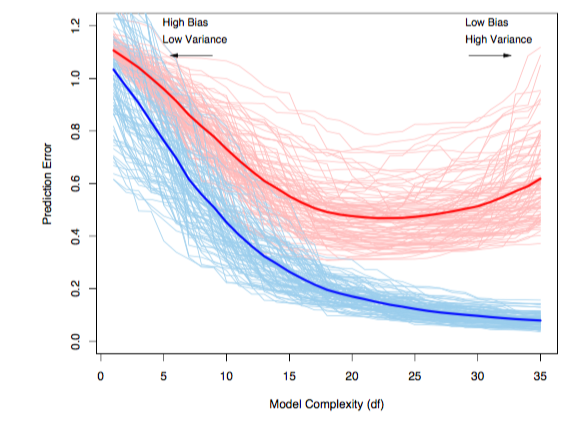
\includegraphics[width=0.7\columnwidth]{figures/figure-biasVariance/figure-biasVariance}
\caption{ Figure borrowed from \protect\textcite{hastie-elemstatslearn} P. 220. Curves are measures of the estimated prediction error for the different degrees of freedom in the model (number of features). Blue curves correspond to the training error and red curves are for the test error. The bold curves are calculated by averaging over all the colored curves.%
}
\label{figure:biasVariance}
\end{center}
\end{figure}


In \cref{figure-biasVariance}, the authors fit a model to illustrate the interaction between bias and variance. The model increases complexity when using a greater number of features. This is because during the optimization procedure, the algorithm has to fit more parameters. Thus, the model increases in complexity, as measured in its degrees of freedom.

As a similar example, we reproduce the previous behavior on our own dataset.
Consider \cref{target2} which has a high imbalance between the positive and negative target classes.
With a Decision Tree classifier, we try to produce a model which overfits $\mathcal{T}$. This model can increase complexity by considering the depth of the tree. Where higher depth means more complex models\footnote{A detailed explanation of this technique can be found later in \cref{section:decision_trees}. }.
To score the model, we take a monotonically increasing scoring function where
higher values mean better scores.
With this, the different model errors produces the following figure. Where the test and training errors are given as a function of the tree\'s depth:

\begin{figure}[h!]
\begin{center}
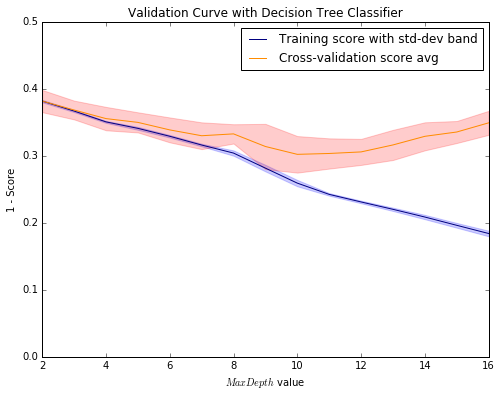
\includegraphics[width=0.7\columnwidth]{figures/figure-biasVariance/dtree_overfit_problem_2.png}
\caption{
}
\label{figure:dtree_overfit_problem_2}
\end{center}
\end{figure}


At first the bias of the model is high both for the training and testing sets, and as a consequence, we would expect to have a high generalization error. Then the overall error decreases as complexity increases. This behavior is expected because the model learns to better fit the data to give a better model output. We have that the expected prediction error, estimated by averaging over the test set' prediction error's, also decreases when the model's complexity is increased. However, when the model starts to overfit the data, the test error starts to rise whilst the train error keeps decreasing. This situation is important to our prediction error estimation cause it hints that the model has lost predictive power due to an increase in variance.

In these situations, the author\'s of \cref{figure:biasVariance} argument that a rough heuristic to select the best model is to stop increasing the model's complexity once the $EPE$ stops decreasing. That is, when the scoring error of the test set stops decreasing along with the training error. In \cref{figure:dtree_overfit_problem_2} this would be when $Max Depth = 10$.

For the examples exposed, we see that we are only finding the best model by searching only on one hyperparameter. In practice, the models will have more parameters to tune. This makes finding the lowest prediction error difficult.
Still, we might settle for near-optimal models which have an acceptable error score. The following section introduces the assumptions to consider the test error as a good approximation of the generalization error. It also gives a formal argument in favor of finding models whose scores are not optimal for that dataset.


\section{ Using the Vapnik-Chervonenkis (VC) Dimension for prediction error estimation}\label{section-VcDimension}

%\textcite{vapnik-nature2013}
%\textcite{cherkassky-learning2007}

In Vapnik and Chervonenkis' work, the focus is on the estimation of the prediction error through the convergence and consistency of the training error. The authors derive the VC dimension as an important value in determining convergence speeds for different machine learning algorithms. In this way, a theoretical framework is provided to effectively characterize these dimensions in a constructive way. By the derived analytic bounds for a number of algorithms, we are enabled to estimate the distance between the empirical error and the generalization error.

The Vapnik-Chervonenkis (VC) Dimension is a number based on a theoretical framework now called \textit{Statistical Learning Theory} (SLT). SLT is used to estimate the true expected prediction error from finite samples. Surprisingly, very few assumptions are needed and the results are distribution independent. In addition, exact bounds are given for some common use cases with constructive analytical methods. For other cases, authors propose sampling or experimental methods to estimate the VC dimension.

For this part, most of the results and reasoning follows the works in \textcite{cherkassky-learning2007}. For a more broad development of this work, \textcite{vapnik-nature2013} is recommended too. Here we present a brief comment on the consistency of the training error with respect to the prediction error and give example bounds for classification learners. In a supervised learning context, we use the empirical training ($\overline{err}$) or test errors ($\overline{err}_{test}$) to estimate the $EPE$.

Let $\mathcal{T} = (\textbf{X},\textbf{Y})$ be a training set of $n$ samples, $Y = \{0,1 \}$ and let $\mathcal {F} = \big \{ f(x,\theta) \mid x \in X, \theta \in \Theta \big \}$ be a class of classifiers where $f_\theta: X \rightarrow Y \, \forall f \in \mathcal {F}$. This is a class of functions with domain over the input dataset $X$ and which are indexed by a parameter $theta$. This parameter will represent the index over the functions in $F$ and it will vary over all possible models attainable by our algorithm.

As an example, in logistic regression, $theta$ can be indexed by the values of each feature's weights $x^p$. The class $F$ will then represent the set of all possible functions from which to select the final model.
%In applications, a learner is fit from a class of functions.

As it was seen before in \cref{ch:machineLearning}, a common problem in supervised learning when a particular learner is fit and then used to predict new values is overfitting. In practice, this is common when $n$ is \textit{small} or when the number of features is \textit{large}.

Incorporating the loss functions directly in the model, SLT looks at functions of the form $Q(t,\theta) \ = \ L(f_\theta(x,y))$. Seen as a two variable function where $t=(x,y)$ represents a sample of input and output data expressed as a random variable, and $theta$ the class index.

SLT theory focuses on functions which seek to minimize a certain functional characterized by the form of the loss function. Here, the $EPE(\theta)$ for any model takes the functional form

\begin{equation}
\begin{split}
EPE(\theta) = & \ \Expect_{\textbf{t}} \left[ Q(t,\theta) \right]\\
= & \int Q(t,\theta) p(t) dt \\
= & \int L(f_\theta(x),y) p(x,y) dx dy
\end{split}
\end{equation}\label{eq:vapnik-risk}

where we let $p(t)$ be the \textbf{true} underlying probability function of the data. For simplicity, in this analysis we will assume the functions $Q$ in the class to be bounded.

However, as it was said before, we only have access to restricted data and we would like to estimate the risk functional for that class with the available training/test error. In this framework, this is what is called the empirical risk:

\begin{equation}\label{vapnik-empiricalRisk}
Err_{train}(\theta) = \sum_{i=1}^n Q(t_i,\theta)
\end{equation}

Note that the learner is estimated directly from the risk functional. The loss function is placed together with the approximating function and takes a strong part in the minimization procedure. On the other hand the unknown true underlying distribution $p(t)$ will not be estimated to minimize the functional and all the effort will be put in directly using the training error as a \textit{good} substitute for the prediction error.


We know that the training error depends on the model learned from the data and in turn, this depends on the sample. Due to this non-deterministic aspect of the problem, we will have different output models for varying input samples, and even sometimes for the same sample. Yet as we increase the sample size, we would still want to have the training error converge and to be consistent with the prediction error of the models.

%and $\theta^{*}_n$


\begin{definition}{Consistency of the Training error}

Let $\{\mathcal {T}_1, \mathcal {T}_2, \ldots, \mathcal {T}_n, \ldots \}$ be a set of training samples such that $\forall n \ |T_n|=n$. Given a training sample of size $n$ and a class of learners $\Theta$, let $\theta^{*}_n$ be the argument minimizing the training error and let $\theta_0$ be the minimizing argument for the prediction error over the class of functions i.e.\ over all the models of the class.

Then, the training error is said to be consistent if

\begin{equation}
\lim_{n\to\infty} Err_{train}(\theta^{*}_n) \ = \lim_{n\to\infty} EPE(\theta^{*}_n) \ = EPE(\theta_0)
\end{equation}

\end{definition}

The property of asymptotic convergence in the training and prediction errors is expected in any learning algorithm. In SLT, the consistency requires that the training and prediction errors' sequences not only converge to the same values, but that the sequence of minimal training errors also converge, to the minimizing value of the prediction error. At the same time, the sequence of prediction errors must converge to this same point.

In reality, it is reasonable to think that the approximation of the prediction error with the training error introduces a strong overestimation. The training error will also be biased by the sample used whilst the prediction error is given for the whole class and is not dependent on the sample. This is very important, since the minimization of the training error when using bounded loss functions is consistent if and only if:

%\begin{definition}{Uniform Consistency of the Training Error}

%\end{definition}
\begin{equation}
\forall \epsilon > 0 \ , \ \lim_{n\to\infty} P\left[ \sup_{\theta \in \Theta} \mid Err^{n}_{train}(\theta) - EPE(\theta) \mid  > \epsilon  \right] = 0
\end{equation}

Here the training error $Err^{n}_{train}(\theta)$ is the value of this error when using a sample of size $n$. In this sense, the training error is said to be consistent if it converges uniformly in probability over the whole class of functions\footnote{Remember that approximating functions in the SLT setting are indexed by the $\theta$ parameter.}. This implies that it characterizes the set of functions $Q(t,\theta)$ used to approximate the data will be important in finding an appropriate model. %SLT theory then introduces

The next results will be focused on a binary supervised machine learning setting. Yet the extension to other forms of supervised learning can be found in \textcite{cherkassky-learning2007}.

\begin{definition}{Shattering}

Let $\mathcal {A}= \{A_1,A_{2},\dots \}$ be a set family and $T$ a finite set. Let $t \subseteq T$, it is said that $\mathcal {A}$ picks out $t$ if there exists $A' \subseteq \mathcal {A} $ such that $ T \cap A' = t$. $T$ is said to be shattered by $\mathcal {A}$ if it picks out all its subsets.

%The VC dimension of $\mathcal {A}$ is the biggest cardinality of a set shattered by $\mathcal {A}$.

\end{definition}

The n-th shattering coefficient $\Delta_n$ of a class $\mathcal {A}$ is defined to be the maximum number of subsets of $n$ elements picked out by the class.

If we consider a function from our set of classifiers, given a training set of size $n$
$\mathcal {T} = \{ t_1,t_2,\ldots,t_n \}$, we know that each classifier acts as an indicator function on the inputs $\{ x_1,x_2,\ldots,x_n \}$. The \textit{diversity} of this set of classifiers intuitively represents all the diverse ways in which the input sample is partitioned by the classifiers.

We would say that $t$ is picked out by $\Theta$ if there exists a classifier $f_{\theta} \in \Theta$ such that $T = f_{\theta}^{-1}(\{1\})$. The classifiers in $\Theta$ define a unique mapping to the class of sets where each classifier is positive. It is said that $\mathcal {F}$ shatters a set $A$ if all its subsets are picked out by the class of functions.

We will now reproduce the main necessary and sufficient conditions to have uniform consistency in predictive error approximation of our defined class of loss functions. Also,
Vapnik et AL provides bounds for the exponential convergence of this error. These bounds are constructive and can be effectively calculated in a number of commonly used models such as linear regressors and support vector machines. In addition, these bounds depend \textbf{only} on the structure of the approximators rather than the true distribution of the data.


\begin{definition}{Vapnik-Chervonenkis (VC) Dimension}

The Vapnik-Chervonenkis Dimension (VC) of a class of binary functions is the cardinality of the largest set which is shattered by $\mathcal {F}$.\footnote{The VC dimension is briefly introduced here for the purpose of giving a theoretical approach to error estimation in machine learning methods. For a complete explanation on this topic, refer to \textcite{vapnik-nature2013}}
\end{definition}


Note that by definition this means that there needs only to exist one set shattered by $\mathcal {A}$, to have the VC dimension at least as big as that set's cardinality.


The VC dimension gives a certain criteria for measuring the complexity of a class of binary functions by evaluating its expressiveness. The value, however, need not be finite.

As a simple example, one could use a linear regression of $d$ features
\begin{equation}
g_{\theta} = \sum_{i=1}^d x_i \theta_i + \theta_0
\end{equation}

 as a classifier if we consider the indicator function of the positive half-plane induced by the regression:

\begin{equation}
f_{\theta} = I(\sum_{i=1}^d x_i \theta_i + \theta_0 > 0)
\end{equation}

This class of approximating functions can shatter up to $d+1$ samples, but no bigger sample. Thus the VC dimension is exactly $d+1$.
 %% EZECORRECTION: dar demostracion o citar a algun lado que la den sobre esto. Induccion sobre la cantidad de puntos arrancando con el caso obvio.

For more examples, refer to \textcite{cherkassky-learning2007} Pg. 113 for examples of different VC classes, finite and infinite.

SLT then proves that if a class of binary classifiers is of finite VC dimension, accurate bounds can be given to estimate train and predictive errors. For a sample of size $n$, take $Err^n_{train}(\theta^*)$ to be the minimum training error and $EPE(\theta_0)$ the minimum true predictive error.

 %% EZECORRECTION: citar a algun lado que la den sobre esto.

They show that for classes which have a finite VC dimension $h$, the n-th shattering coefficient is bounded by a polynomial of order equal to the dimension
i.e.\ $\Delta_n(\mathcal {F}) \leq O(n^{h})$,\footnote{$O(\cdot)$ corresponds to Big-O notation.}.
 %% EZECORRECTION: citar a algun lado que la den sobre esto.


 %% EZECORRECTION: explicar mejor la relacion entre eta, que es algo que se elije, y n para la cota + grado de confianza que vos necesitas para saber cual es el intervalo de confianza, etc.

Also, we can define $\eta \in (0,1)$ to have that with probability at least $1 - \eta$ and $\forall \theta \in \Theta$

\begin{equation}
EPE(\theta) \leq Err^n_{train}(\theta) + \frac{\epsilon}{2} \left(1 + \sqrt{1 + \frac{4 Err^n_{train}(\theta) }{\epsilon}} \right)
\end{equation}\label{eq:vapnik-classificationBound}

, and when the approximating class $F$ is infinite of size $N$:

\begin{equation}
\epsilon = a_1 \frac{h \left( \ln(\frac{a_2 n}{h} ) - \ln(\frac{\eta}{4} ) \right)}{n}
\end{equation}\label{eq:vapnik-epsilonBound}

or

\begin{equation}
\epsilon = 2 \frac{ \ln(d) - \ln(\eta)}{n}
\end{equation}\label{eq:vapnik-epsilonBoundSimple}

when $F$ is finite and consists of $d$ elements.

In the preceding equations, the values of constants $a_1$ and $a_2$ are related to the nature of the density function $p(t)$ of the data. However, its values are proven to be uniformly bounded for all distributions, with $a_1 \in {(0,4 ]}$ and $a2 \in {(0,2 ]}$.

As a last result, the authors show that a more precise bound can be given for the function that minimizes the empirical risk $Err^n_{train}(\theta^*)$. They show that with probability $1 - 2\eta$

\begin{equation}
Err^n_{train}(\theta^*) - EPE(\theta_0) \leq \sqrt{\frac{-\ln(\eta)}{2n} } + \frac{\epsilon}{2}\left( \sqrt{1 + \frac{4}{\epsilon} } \right)
\end{equation}\label{eq:vapnik-classificationBoundPrecise}

These results prove that effective approximations of the prediction error can be given for most algorithms of finite VC dimensions. They also give a distinct characterization of how model complexity is related to the prediction error estimation.

In practical applications though, use of estimates might be limited to the determination of the VC value, specially with algorithms which are more complex and expressive such as neural networks. Due to this limitation, we show in the next section a practiced approach which is an easier and direct heuristic used to estimate the $PE$.


\section{Cross Validation}\label{section:crossValidation}

 There are a number of approximating functions or algorithms to be used in classification problems and each of these have different configurations or setups that, when fitted, produce different learners. The differences between the configurations are controlled by the \textit{parameters} of the algorithm. The nature of each parameter might stem from computation or statistical variants in the algorithm used. One common example of this is the $\lambda$ penalization parameter in logistic regressions, where $\lambda$ controls the amount of weight to be placed on the regularization term of the minimized function.

The objective of Cross Validation is to systematically explore the different configurations of tuning parameters and decide which learner is better for the task at hand. By comparing the estimated generalization error of each model, where models vary accordingly with the values of the tuning parameters, a value is given and then used to select the \textit{best} model in the class.

This technique is considered one of the most widespread to evaluate the generalization performance of a set of learners. Given a number of possible configurations or values for the tuning (hyper) parameters of an algorithm, we would want to decide which selection of these fit the best estimator, as measured by the generalization error.

In terms of the concepts introduced before, the quality of an estimated model $\hat{f}$ from a family of algorithms is evaluated in the Cross Validation procedure. Where quality refers to the rate of generalization error.

In most cases data is generally scarce. At the same time prediction error estimates are based on asymptotic or analytical results which hardly computable in practice Thus CV intends to prevent over-fitting by iteratively holding out a random part of the dataset and by measuring the predictive accuracy of the learner fit of data \textit{in-sample} against new values from the \textit{hold-out} part of the dataset. The accuracy measure here is weighted by the loss function, which must be selected beforehand.

In this procedure, a partition of the samples is called a \textit{fold}. CV then partitions the data into $K$ random separate sets or  \textit{folds}, where the number $K$ has to be previously decided.\footnote{ We assume here that a random sample of the initial dataset was already left out in order to test the model's accuracy at the end. We refer to this set as the \textit{testing set}.} Let $\gamma : \{1,..,N\} \mapsto \{1, .., K\}$ be a function mapping samples to folds. Without loss of generality, let $\alpha$ be an index of the model's hyper-parameters, where each distinct combination of the tuning parameters is identified by this index. Note that the domain of $\alpha$ will vary with the type of approximating function o algorithm used to learn.

 The CV algorithm now runs iterations over all the folds, and takes one fold $\gamma^{-1}(\{k\})$ to be the validation set, where $k \in [1,\ldots,K]$ is the indexer of the iteration. $\hat{f}^{-k}$ will denote the fitted estimator on the training set with the $k$-fold hold out and its classification performance will be tested against the \textit{out of sample} estimates. This means that for every sample in this $k$-fold, we measure the loss $L(y_i, \hat{f}^{-\gamma(i)}(x_i))$ of the model's prediction against the true target value.

Cross validation intends to estimate the expected \textit{out-of-sample} error $\Expect \left[ L(Y, \hat{f}(X)) \right]$, when the model is tested against \textbf{independent} samples from the true distribution. For this reason, it is fundamental to ensure independence of the training set and the test set. Any transformations that must be done on the input data that jointly use the input and output samples in the process must be done and \textit{learned} only on the training set. This is because we mustn't introduce information from our test set in the estimator as the model should never \textit{see} the test data until we use it to evaluate our learner.

\subsection{Selection of tuning-parameters (hyper-parameters) }\label{subsection:selection_hyper_params}

 Let $\mathcal{A} = [\alpha_0, \alpha_1,\ldots, \alpha_l  ]$ be a list of hyperparameter settings and $\mathcal{K} =[1,..,K]$ a list of folds. A full K-Fold Cross Validation procedure takes the following form.

 \begin{algorithm}%[h]
 \SetAlgoLined\KwResult{Data table mapping error scores $CV(\alpha) \ \forall \alpha$}
 Initialize $\mathcal{A}$ and $\gamma(\cdot)$\;
 \For{ $\alpha \in \mathcal{A}$}{
 \If{data transformation}{
 Perform data transformation on the whole training set \;
									 }
 \For{ $k \in \mathcal{K}$}{
 	 \If{feature selection}{
 	 	Perform feature selection on the $\textrm(T)^{-k}$ \;
 	 }
 fit $\hat{f}^{-k}(\cdot, \alpha)$\;
										}
 compute $CV(\alpha) = \frac{1}{N} \sum^n_{i=1} L\left( y_i, \hat{f}^{-\gamma(i)}(x_i, \alpha) \right)$\;
												}
 \caption{K-Fold Cross Validation Estimation Procedure}
 \end{algorithm}

Note that during the loop for $\alpha$, each sample's prediction is tested on the model which was fitted without using that sample same sample.
This is central to the idea of cross-validation in which training samples are used \textit{as if} they were testing samples.
For this reason, samples that are not used to train the model are called validation samples.

From the \textbf{CV} procedure, it makes sense to choose a final model $\hat{f}_\alpha$ with the lowest $CV(\alpha)$ value among all possible hyperparameters. However, following ideas detailed in \cref{section-VcDimension}, importance should also be given to the \textit{complexity} of the approximating function. A common rule of thumb is to favor models with a lower number of hyper parameters or number of features. In practice however, a class of approximating functions might have a defined complexity which is not analytically computable. Thus in some cases, crude heuristic estimates or common sense is used to estimate model complexity, without making use of theoretical arguments.


As an example, we consider here a cross validation procedure done on a logistic regression model. The hyperparameter to search is the $C = \frac{1}{\lambda}$. Recall from \cref{eq:logitRegularization} that this is the regularization strength of the model, where a smaller value in $C$ meant a stronger regularization. We perform this experiment and consider the difference in errors for $$
In figure

\subsection{Choice of \texorpdfstring{$K$ parameter}{Lg} }

 Experimental results show the differences among CV routines used with varying $K$ number of folds. In synthetic and actual dataset~\textcite{hastie-elemstatslearn} P. 243, have found that using a \textit{higher} value of $K$, relative to the size of the dataset, means having a bigger training fold since each left-out partition is only $\frac{N}{K}$ in size. The results show models with good bias but high variance, which is in conformity with the small size of the validation set. Note that having a higher value for $K$ will effect to a higher computational burden since $K$ estimators need to be fitted.

Having a lower $K$ value means using a smaller training set. Then it is common to find models with lower variance and higher bias. Empirical results suggest that to show that the $EPE$ is overestimated. This is because having less available data to fit the model, implies having worse estimates from asymptotic results.

One last common choice for $K$ is $N-1$. This scenario is known as \textit{leave-one-out CV} and is a very used format for problems where data arrives sequentially over time. Here, samples of the training set $t_i = ( \boldsymbol{x_i} , \boldsymbol{y_i} )$ are accessible only in an orderly fashion. For these cases model evaluations are made against the new sample and the training set is updated with every arrival.\footnote{Note that here we must assume samples to be \textit{exchangeable}. This means that the training set distribution is not altered by a permutation of samples $F(x_1,\ldots,x_n ) = F(x_\sigma{1},\ldots,x_\sigma{n})$ for any random permutation $\sigma$.}

 %% EZECORRECTION: agregar aca un ejemplo en el cual reentrenar una cosa que ya tenes entrenada agregando solo 1 punto o una cantidad de puntos es mucho mas rapido hacer un pequenyo update que reentrenar con todos los puntos.


A valuable survey and explanation of the drawbacks of the $K$-Fold CV estimator can be found in \textcite{bengio-unbiasedCvEstimator}. The authors prove that there is no distribution-free estimator unbiased estimator of the $K$-Fold cross validation estimator's variance. The theoretical arguments focus on the idea that error correlations between the training and validation sets are not taken into account by the CV procedure. These correlations are known and understood for the general case, but their estimation is not possible. As a consequence of this, comparison between different possible models are hindered.

Empirical examples are built from synthetic datasets to show the shortcomings of the cross validation's algorithm which might show high deviations from its central value. Some exceptions appear though, specifically where distribution-free bounds can be found for a class of approximating functions. But these cases are specific only for this class. In general, these bounds are not known, so using an unknown deviation of the CV estimator will affect the evaluation of different models.

Consensus\footnote{\textcite{hastie-elemstatslearn} P. 260} is that in general CV is a good procedure to estimate the expected prediction error with the training set fixed, but not good for the prediction error, conditional on the training set $\mathcal{T}$ fixed.



\subsection{CV Scores in Classification Learning}\label{section:scoring_functions}

In binary classification, the contingency table summarizes all of the learner's training performances. This shows the count of the amount of samples that fall into one of the four groups derived from the comparison between the model's output and the observed data for the labels.

 Let $\hat{f}$ be our fit model, from the data with a CV procedure. Every sample has a target value $y$ and a predicted outcome $\hat{y}$ and there are only four possible interactions of these two variables for two values each. We can express the models' target outcomes $\hat{y}$ into the positive ($\hat{P}$) or negative ($\hat{N}$) categories and the same with actual target data into the positive ($P$) or negative ($N$) categories.

To assess the performance of the classification algorithm and chose the \textit{best} model we must decide on how the CV procedure will value two different models. The idea is to quantify the mismatch between the target and the predicted value. Here loss functions are also known as \textit{scores}, \textit{measures} or \textit{utility functions} and are built by looking at how many times an algorithm misclassifies instances and where is the misclassification happening. To visualize this the \textit{confusion} table presents these results in the following draft:

\noindent
\renewcommand\arraystretch{1.5}
\setlength\tabcolsep{0pt}
\begin{tabular}{c >{\bfseries}r @{\hspace{0.7em}}c @{\hspace{0.4em}}c @{\hspace{0.7em}}l}
\multirow{10}{*}{\parbox{1.1cm}{\bfseries\raggedleft\ Target\\ value $y$}} &
& \multicolumn{2}{c}{\bfseries Predictive value $\hat{y}$} & \\
& & \bfseries \^{P} \ $(0)$ & \bfseries \^{N} \ $(1)$  \\
& P \ $(0)$ & \MyBox{True}{Positive (TP)} & \MyBox{False}{Negative (FN)} & \\[2.4em]
& N \ $(1)$ & \MyBox{False}{Positive (FP)} & \MyBox{True}{Negative (TN)} & \\
%& total & P \ $(0)$ & &
\end{tabular}

In the confusion table, cell values count the amount of instances that fall into each of the four possible outcomes. From this metrics scores are constructed to provide values on the algorithm's performance. Different interactions of these counts can measure different aspect's of an algorithm's classification performance.

%Their focus is in measuring $FP$ and $FN$ volumes.

% to measure the algorithm's performance.
% Notice that the only correct cells are the $TP$ and $TN$ categories, each correctly classifying positive and negative samples
Some of the most used metrics include the following:

\begin{itemize}
\item \textbf{True Positive Rate (Recall):} $\frac{TP}{P} = \frac{TP}{TP + FN}$ \\ This rate measures the percentage of real positive values captured by the algorithm. A high recall of the algorithm indicates that a high number of the real positive labels were classified as positive.


\item \textbf{Positive Predictive Value (Precision):} $\frac{TP}{\hat{P}} = \frac{TP}{TP + FP}$ \\ This rate measures the \textit{confidence} of the algorithm in its positive predictions, where a high precision indicates value in its predictions.

\item \textbf{True Negative Rate (Specificity):} $ SPC = \frac{TN}{N} = \frac{TN}{TN + FP}$ \\ This rate measures the percentage of real negative values captured by the algorithm.


\item \textbf{False Positive Rate (Fall-Out):} $FPR = 1 - SPC$ \\ This rate measures the percentage of false negative values misclassified by the algorithm.

\item \textbf{Accuracy:} $\frac{TP + TN}{P + N} = \frac{TP + TN}{TP + FP + TN + FN}$ \\ This rate measures the \textit{confidence} of the algorithm in all of its predictions.

%\item $F1_\beta$ \textbf{Score:} $(1 + \beta^2) \frac{TP + TN}{P + N} $ \\ This is the harmonic mean of the recall and the precision. It's advantage is that it can capture both of the scores in equal weight. Its values range in the $\[0,1 \]$ domain and are ordered in the sense that perfect classifiers have a $F1$ score of 1.
%
\item \textbf{F1 Score:} $\frac{TP + TN}{P + N} = \frac{TP}{TP + FP} = 2 \frac{1}{ \frac{1}{recall} + \frac{1}{precision} }$ \\ This is the harmonic mean of the recall and the precision METRICS.\@ It's advantage is that it can capture both of the scores in equal weight. Its values range in the ${[0,1 ]}$ domain and are ordered in the sense that perfect classifiers have an $F1$ score of 1.

\end{itemize}


\todo{show an instance of problem comparing all metrics}

\subsection{ROC Curve}

One last important metric used widely in classification is the \textbf{Area under ROC curve (ROC AUC)}. This metric applies only to algorithms which output for each sample the probability of belonging to the positive class.

With these algorithms we would have that the output target will be defined as

\begin{equation}
\hat{y} =
\begin{cases}
&1 \ \mbox{if} \ f(x) > \pi \\
&0 \ \mbox{else}.
\end{cases}
\end{equation}

where $\pi$ is a threshold value which will separate positive from negative samples. If we consider different values for $\pi$, we will see that the recall $R$ and the fall-out $FPR$ of the algorithm will vary accordingly. We can then define the ROC curve to be

\begin{equation}
\sigma(\pi) = (R_\pi, FPR_\pi)
\end{equation}

As expected, there is an inverse relationship between these two as the threshold is varied. The result is a curve defined in $[0,1]\times[0,1]$, referred to as the \textit{ROC space}.

To find a balance between these two rates, the ROCAUC metric measures the integral of this curve in ROC space. The score calculated is thus known as \textit{Area Under the ROC Curve}. This metric follows the same properties as the ones mentioned before, where the best classifiers have values nearer to $1$.\footnote{As a side note, the ROC AUC measure is proportional to the statistic of the Mann-Whitney U-test, where the means of the classifier's output positive and negative classes are compared. More information on this can be found in \textcite{mason-rocAucRelationship}.}



The following figure is an example ROC curve for an instance problem. Notice the algorithm's poor prediction performance where the ROCAUC is barely over the `Luck' line. This line constitutes the performance of a \textit{random} classifier which arbitrarily labels samples as being to each possible class. It is expected to see good learners have better ROCAUC scores than the \textit{random classifier}.

\begin{figure}[h!]
\begin{center}
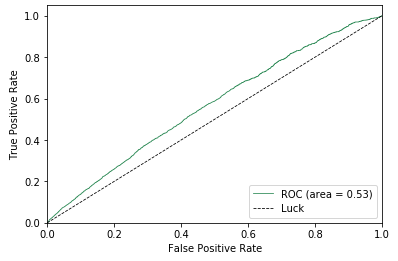
\includegraphics[width=0.7\columnwidth]{figures/figure-lowROCAUC/figure-lowROCAUC_original}
\caption{Example of a ROC curve from a Random Forest classifier used on the \textit{cancer} dataset. The code used to build this graph is largely based on Python's Sci-kit Learn library. \protect\footnote{For more information on `sklearn' please refer to \url{http://scikit-learn.org/stable/index.html} \protect\textcite{scikit-learn}. The cancer dataset is a copy of the UCI ML Breast Cancer Wisconsin (Diagnostic) set and is available from this same module or from \url{https://goo.gl/U2Uwz2}.} }
\end{center}
\end{figure}\label{fg:lowROCAUC}
%

As a counter example, another algorithm was run on the same problem as \cref{fg:lowROCAUC}.Notice how the algorithm is considered \textit{perfect} by the ROCAUC metric. No data transformation has been applied to the set between runs. The difference in the two scores is notable and corresponds entirely to the algorithm chosen.\footnote{The code used for this run can be found in a public iPython Notebook accessible at \url{https://github.com/jdemonasterio/authorea/blobster/Notebooks/roc_curve_graph.ipynb}}

\begin{figure}[h!]
\begin{center}
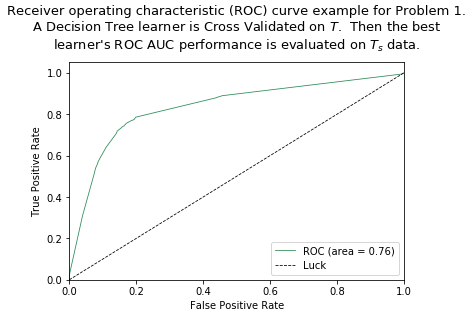
\includegraphics[width=0.7\columnwidth]{figures/figure-highROCAUC/figure-highROCAUC}
\caption{Example of a ROC curve from a Support Vector Machine classifier. The $0.97$ ROCAUC score given is now almost perfect for this problem.%
}
\end{center}
\end{figure}

\todo{add positive ROC concrete example on one of the problems}
